\documentclass{article}

\setlength{\evensidemargin}{0in} \setlength{\oddsidemargin}{0in}
\setlength{\textwidth}{6.7in} \setlength{\topmargin}{-1.1in}
\setlength{\textheight}{10.5in}

\usepackage{amssymb, amsthm, amstext, amsxtra, amsmath, amsfonts, amscd }
\usepackage{graphicx, epsfig}
\usepackage{comment, color, cleveref, listings, wrapfig}
 
\definecolor{dkgreen}{rgb}{0,0.6,0}
\definecolor{gray}{rgb}{0.5,0.5,0.5}
\definecolor{mauve}{rgb}{0.58,0,0.82}
\definecolor{backcolour}{rgb}{0.95,0.95,0.92}

\lstdefinestyle{mystyle}{ frame=tb, backgroundcolor=\color{backcolour}, 
language=R, aboveskip=3mm, belowskip=3mm, showstringspaces=false,
columns=flexible, numbers=none, keywordstyle=\color{blue}, tabsize=3,
numberstyle=\tiny\color{gray}, commentstyle=\color{dkgreen},
stringstyle=\color{mauve}, breaklines=true, breakatwhitespace=true}
\lstset{style=mystyle}

\def\E{\mathbb{E}}
\def\pr{\mathbb{P}}

\renewcommand\baselinestretch{1.2}

\DeclareMathOperator{\sign}{sign}
\DeclareMathOperator{\supp}{supp}

\DeclareMathOperator{\Cov}{Cov}
\DeclareMathOperator{\Var}{Var}
\DeclareMathOperator{\corr}{corr}

\author{Salvador Garcia, s1655274}
\date{10 February 2016}
\title{Assgn3: Students' goals}

\begin{document}

\maketitle
\section{Description of the problem} 

229 students aged 7-13 from 9 schools were asked whether popularity or sporting ability was
most important to them. The aim is to create an appropriate model that takes into account
variability between the schools (if necessary).

\textbf{Statistical analysis.}
Introduce the following random variables. Consider the ith student, $i = 1, 2, ... ,N = 229$, and set $Zi = 1$ if popularity is more important to the student than sporting ability, and $Zi = 0$
otherwise.
\section{Likelihood}
$Z_i | \theta_k \sim Bern(\theta_k)$, where k is the number of the school the ith student is from, independently given $\theta_k$, $\theta_k \in (0, 1)$, $k = 1, 2, ... , 9$.

\section{Prior case 1: $\theta_1 = \theta_2 = ... = \theta_9$}
In this case, each parameter corresponding to the 9 schools are assumed identical. Also, each one of these have a non-informative prior distribution.




\section{Prior case 2: with independent non-informative priors}
\section{Prior case 3: with a hierarchical exchangeable priors}
The data have the following distribution:




The purpose of this assignment is to determine if there is a difference between $\mu_1$ and $\mu_2$. In terms of the problem, to find if there is a relevant difference of gene expression in the two different tissues. In traditional statistics, this can be addressed by testing the hypothesis $\mu_1 = \mu_2$ or, equivalently, $\mu_1- \mu_2 = 0$ given some $\alpha$. In Bayesian statistics something similar can be done, but it is in terms of the posterior distribution of $\delta = \mu_1 - \mu_2$. 
\section{Prior distribution}

\subsection{Priors for $\mu_i$}
In this example we are working with normal distributions (that have two parameters) of two populations , $\mu_1$ and $\sigma_1$ for the first one and $\mu_2$ and $\sigma_2$ for the second one. In order to address the information of the $\mu_i$ parameters, two uninformative priors for $\mu_1$ and $\mu_2$ will be used: $\mu_i \sim N(0, A^2)$ with $A$ very big. This way, the prior distribution of $\mu_1$ and $\mu_2$ will be as the \cref{fig:fig1}. It is easy to see that this distribution assigns almost evenly the probabilities to all values from $(-\infty, \infty)$. Then, can be viewed as non-informative (The idea of apriori with a very big variance is important in this assignment).

Now, given the priors of $\mu_1$ and $\mu_2$, is necessary to think about the priors of $\sigma_1$ and $\sigma_2$. Is important to first give the priors $\mu_i$ because $\sigma_i$ depends on its value. 

\subsection{Priors for $\sigma_i$}
For $\sigma_1$ and $\sigma_2$ a gamma distribution with parameters \textit{shape($\alpha$) = .001} and \textit{rate ($\beta$) = .001} will be used. This distribution is shown in \cref{fig:fig1}. Remembering, the mean of the gamma distribution is $\frac{\alpha}{\beta}$, and the variance is $\frac{\alpha}{\beta^2}$. Then this distribution have $mean = 1$ and $variance = 1000$.

\begin{figure}[ht!]
  \centering
  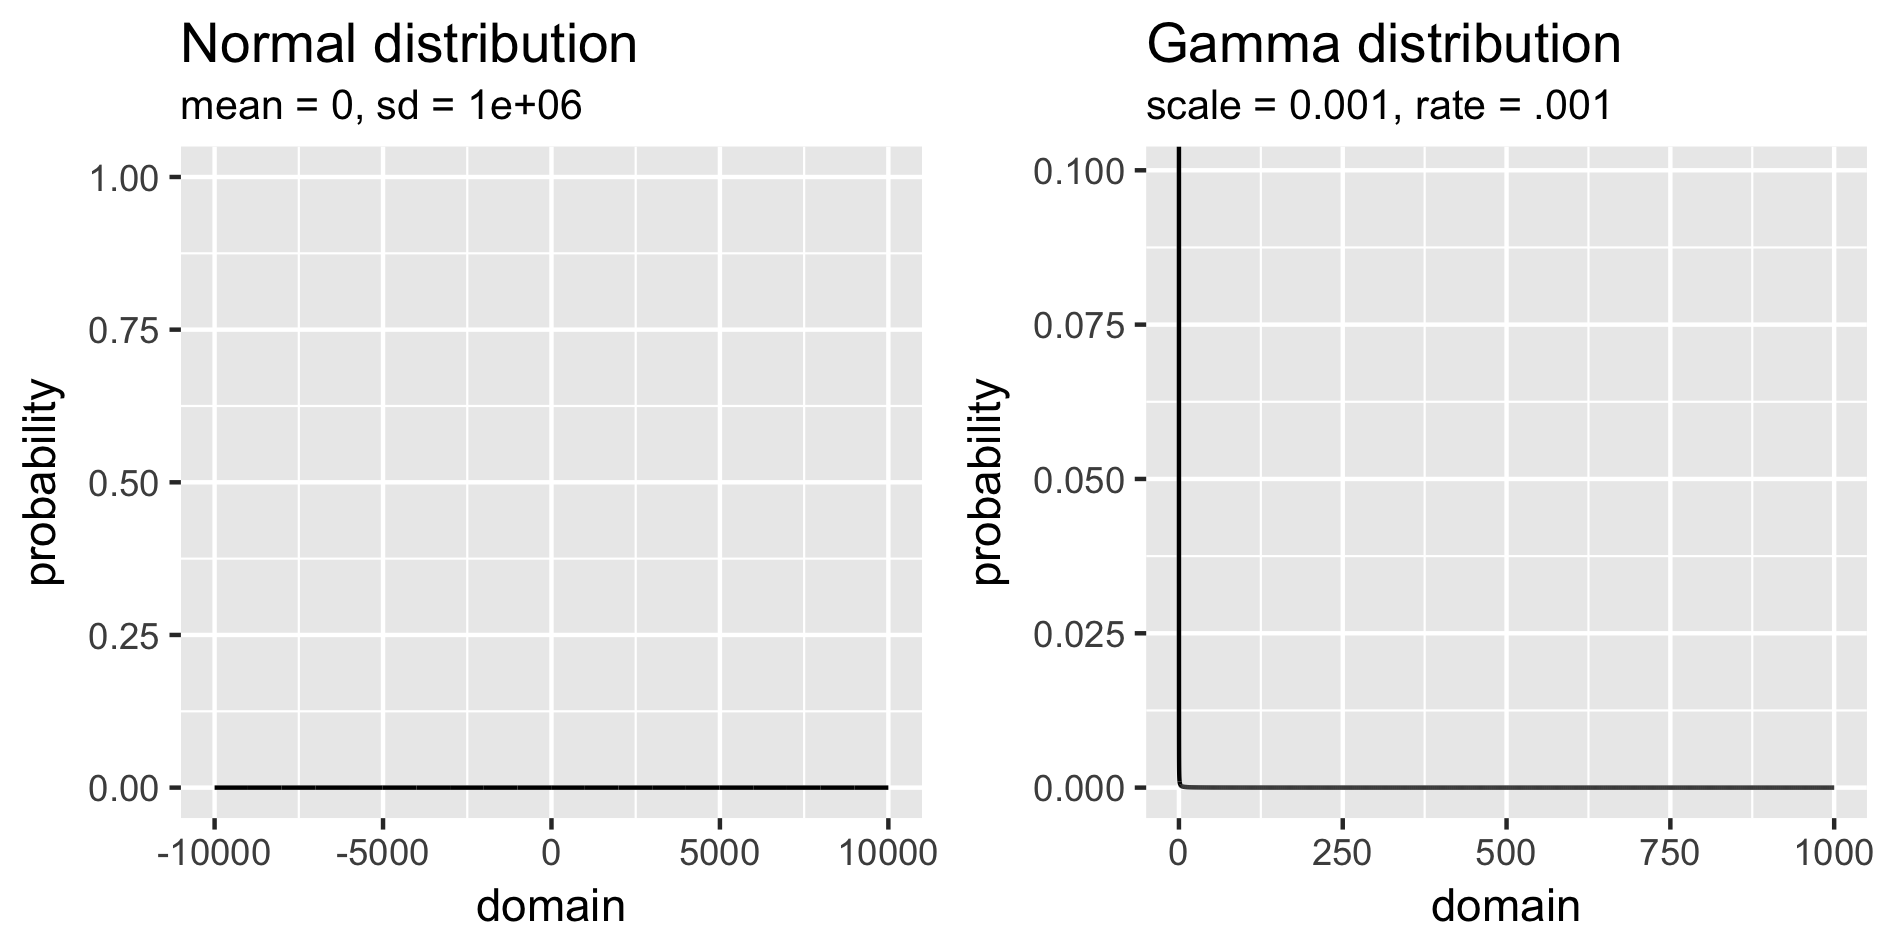
\includegraphics[width=.8\textwidth]{imgs/00_prior_norm.png}
  \caption{Uninformative normal and gamma distributions}
  \label{fig:fig1}
\end{figure}

Now, information from a previous study is used as a new apriori for $\sigma_i$. For the first one, the study says that the average precision (inverse of variance) is 11.11 for the cases and 100 for the control, but the variability is not known. This information given is presented below \cref{eq:1}.

\begin{equation} \label{eq:1}
\frac{\alpha_1}{\beta_1} = 11.11 \qquad,\qquad \frac{\alpha_2}{\beta_2} = 100
\end{equation}

Now, the variability of these values it is not known, so two assumptions to get two different scenarios will be made. The first one is that the prior variance is $10$ and the other that the prior variance is $1000$. Then, for both scenarios, this information can be interpreted as follows\cref{eq:2}:

\begin{equation} \label{eq:2}
\frac{\alpha_i}{\beta_i^2} = 10 \qquad,\qquad \frac{\alpha_i}{\beta_i^2} = 1000
\end{equation}

With these formulas, a system of equations can be created to find $\alpha_1$, $\alpha_2$, $\beta_1$, and $\beta_2$. Using simple algebra, is easy to find that the parameters for the large variance scenario are \cref{eq:3} and for the low variance scenario are \cref{eq:4}.

\begin{equation} \label{eq:3}
\alpha_1 = \frac{11.11^2}{1000}\quad,\quad \beta_1 = \frac{11.11}{1000}\quad,\quad \alpha_2 = \frac{100^2}{1000}\quad,\quad \beta_2 = \frac{100}{1000}
\end{equation}

\begin{equation} \label{eq:4}
\alpha_1 = \frac{11.11^2}{10}\quad,\quad \beta_1 = \frac{11.11}{10}\quad,\quad \alpha_2 = \frac{100^2}{10}\quad,\quad \beta_2 = \frac{100}{10}
\end{equation}

This two \textit{apriori} distributions are used along with the non-informative distribution selected. As the hint says, it is important to distinguish the difference between precision and variance in the model. The one that is modelled though a gamma distribution is the precision. So the variability (variance) of $10$ and $1000$ shown in this section is the variability of the gamma distribution (the prior) of the precision.

\newpage
\section{Posterior inference}
In this section the posterior analysis of $(\sigma_1, \sigma_2)$ will be given. This is done with the relations  $\sigma_1 = \frac{1}{\tau_1}$ and $\sigma_2 = \frac{1}{\tau_2}$. For this analysis, two chains will be used with different initial points (due to the convergence property, at the end both chains will end in the same value).

\subsection{Posterior distributions}
\subsubsection{non informative prior}
\begin{table}[ht!]
\centering
\caption{Summary of analysis with non informative prior}
\label{tbl:1}
\begin{tabular}{llllll}
\hline
parameters & mean   & sd     & 2.5\%  & 50\%   & 97.5\% \\ \hline
$\mu_1$    & 4.03   & 0.0119 & 4.007  & 4.03   & 4.053  \\
$\mu_2$    & 2.59   & 0.005  & 2.58   & 2.59   & 2.6    \\
$\delta$   & 1.44   & 0.0129 & 1.415  & 1.44   & 1.465  \\
$\sigma_1$ & 0.2907 & 0.0084 & 0.2749 & 0.2905 & 0.3081 \\
$\sigma_2$ & 0.1105 & 0.0035 & 0.1038 & 0.1104 & 0.1175 \\ \hline
\end{tabular}
\end{table}

\begin{figure}[ht!]
  \centering
  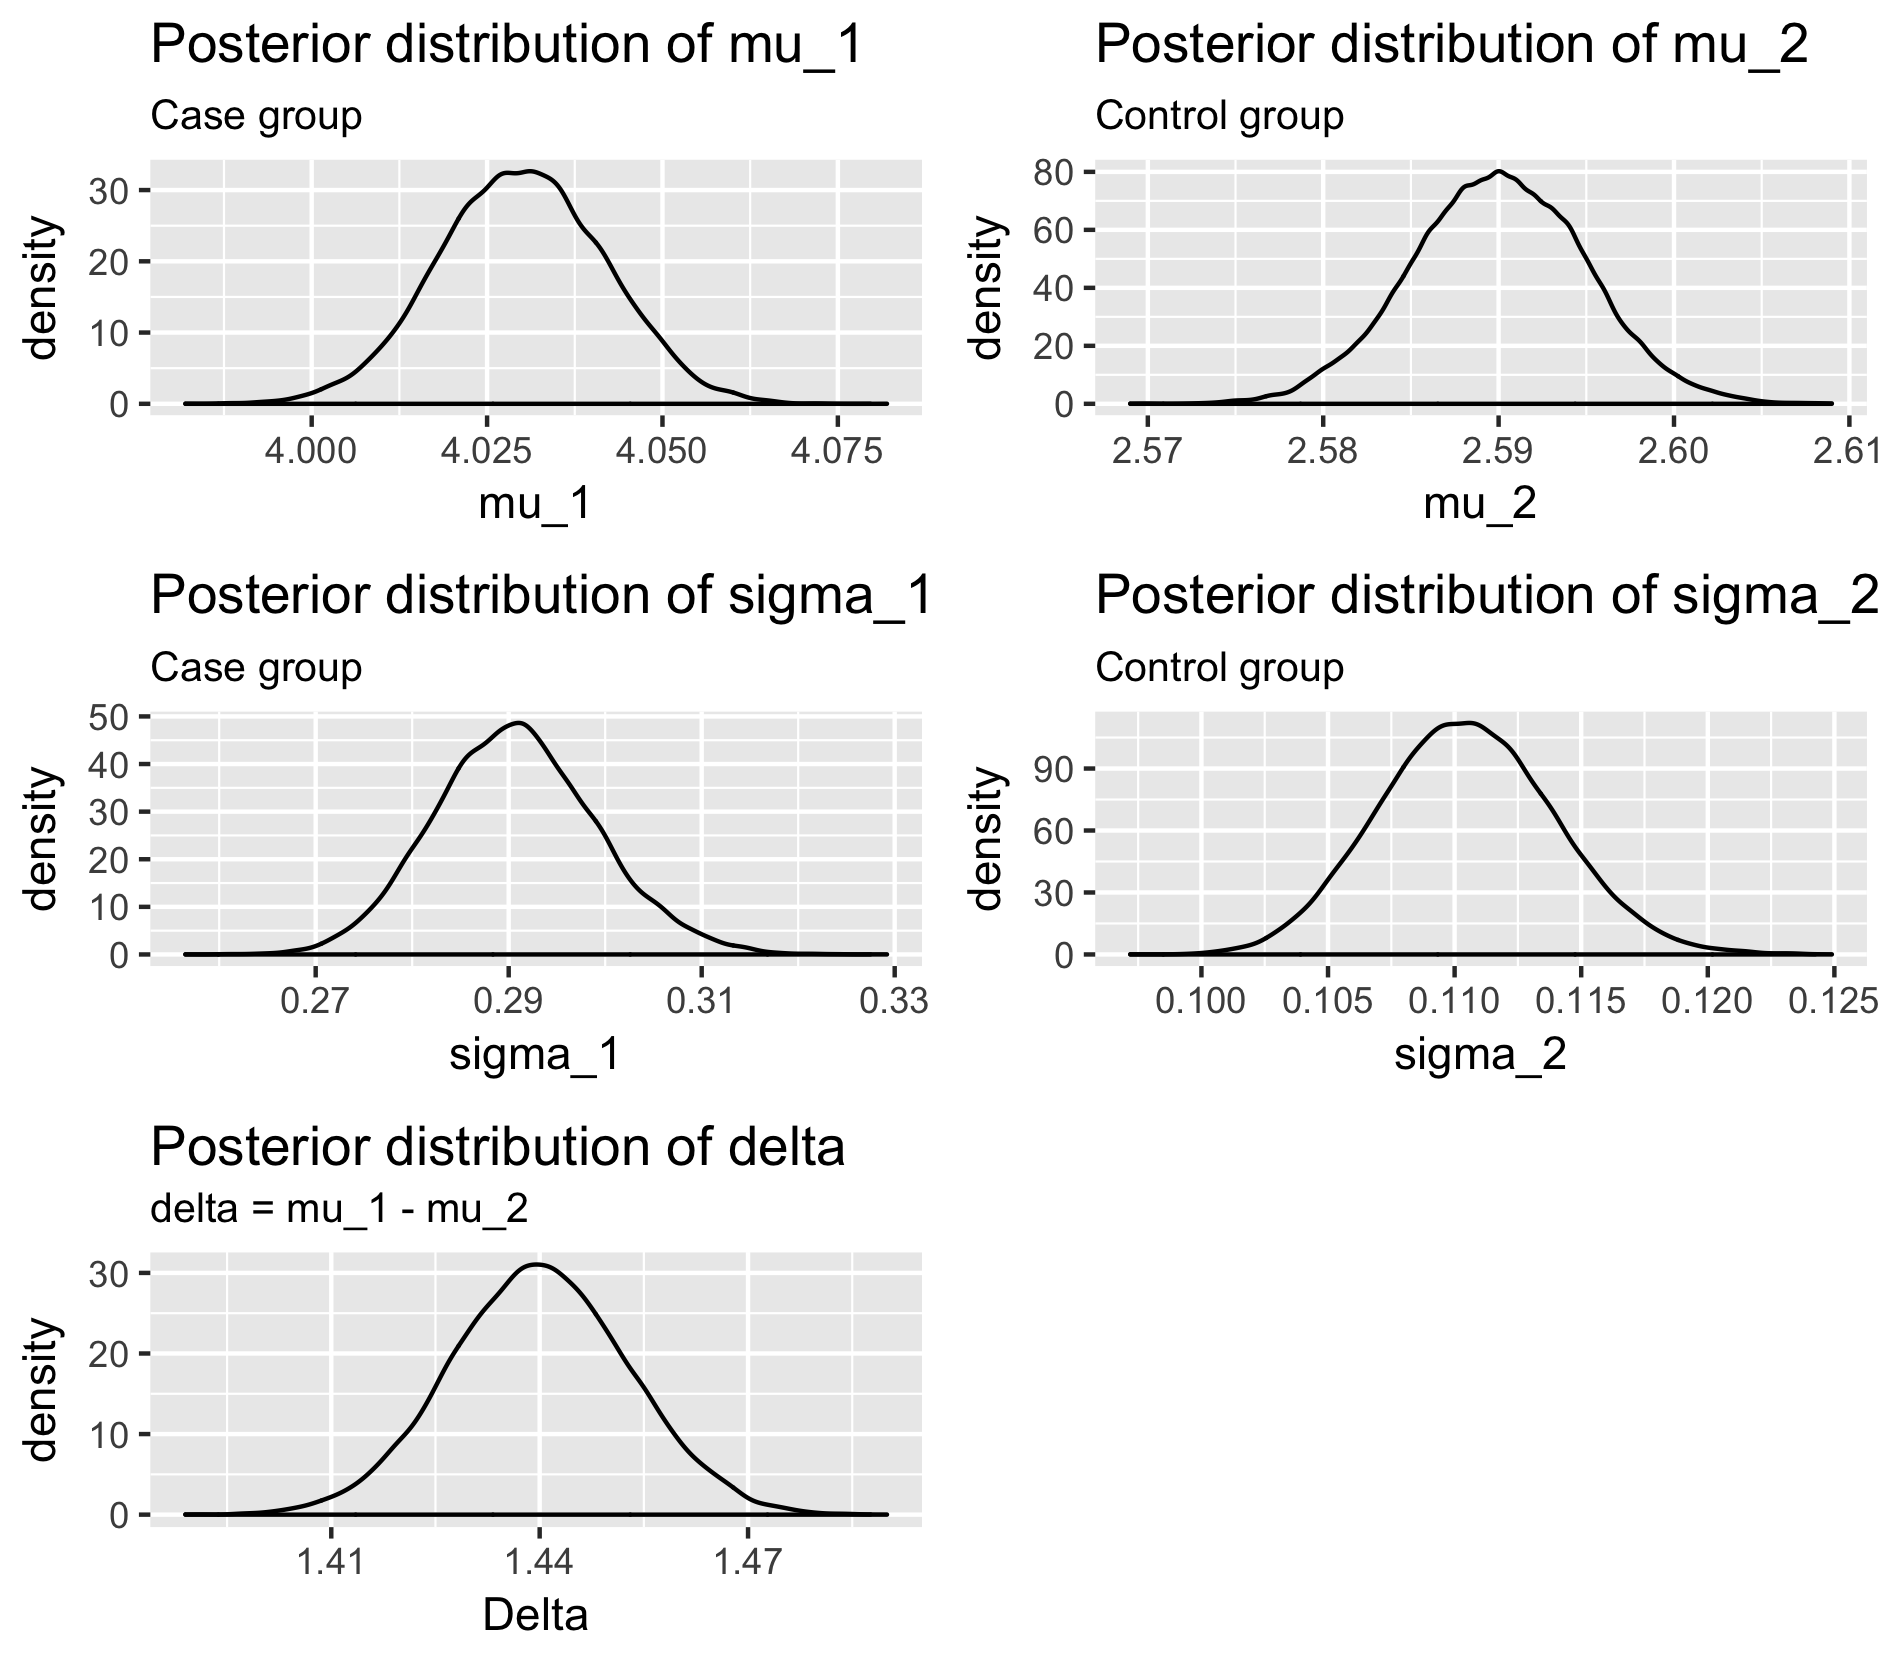
\includegraphics[width=.8\textwidth]{imgs/01_posterior_pars.png}
  \caption{Posterior distributions with uninformative prior}
  \label{fig:fig2}
\end{figure}

In this example, as the \cref{fig:fig2} and \cref{tbl:1} show, there is an important difference between $\mu_1$ and $\mu_2$. In fact, the credibility intervals (95\%) of each are $(4.007, 4.053)$ and $(2.58, 2.6)$ and equivalently for $\delta$: $(1.415, 1.465)$. With this prior, we can conclude that there is a difference between $\mu_1$ and $\mu_2$.

\newpage

\subsubsection{Informative prior with low variance}
\begin{table}[ht!]
\centering
\caption{Summary of analysis with informative prior (low variance)}
\label{tbl:2}
\begin{tabular}{|l|lllll|}
\hline
parameters & mean   & sd     & 2.5\%  & 50\%   & 97.5\% \\ \hline
$\mu_1$    & 4.0299 & 0.0119 & 4.007  & 4.03   & 4.053  \\
$\mu_2$    & 2.59   & 0.0046 & 2.581  & 2.59   & 2.599  \\
$\delta$   & 1.4399 & 0.0128 & 1.415  & 1.44   & 1.465  \\
$\sigma_1$ & 0.291  & 0.0082 & 0.2755 & 0.2909 & 0.3081 \\
$\sigma_2$ & 0.1021 & 0.0014 & 0.0994 & 0.1021 & 0.105  \\ \hline
\end{tabular}
\end{table}

\begin{figure}[ht!]
  \centering
  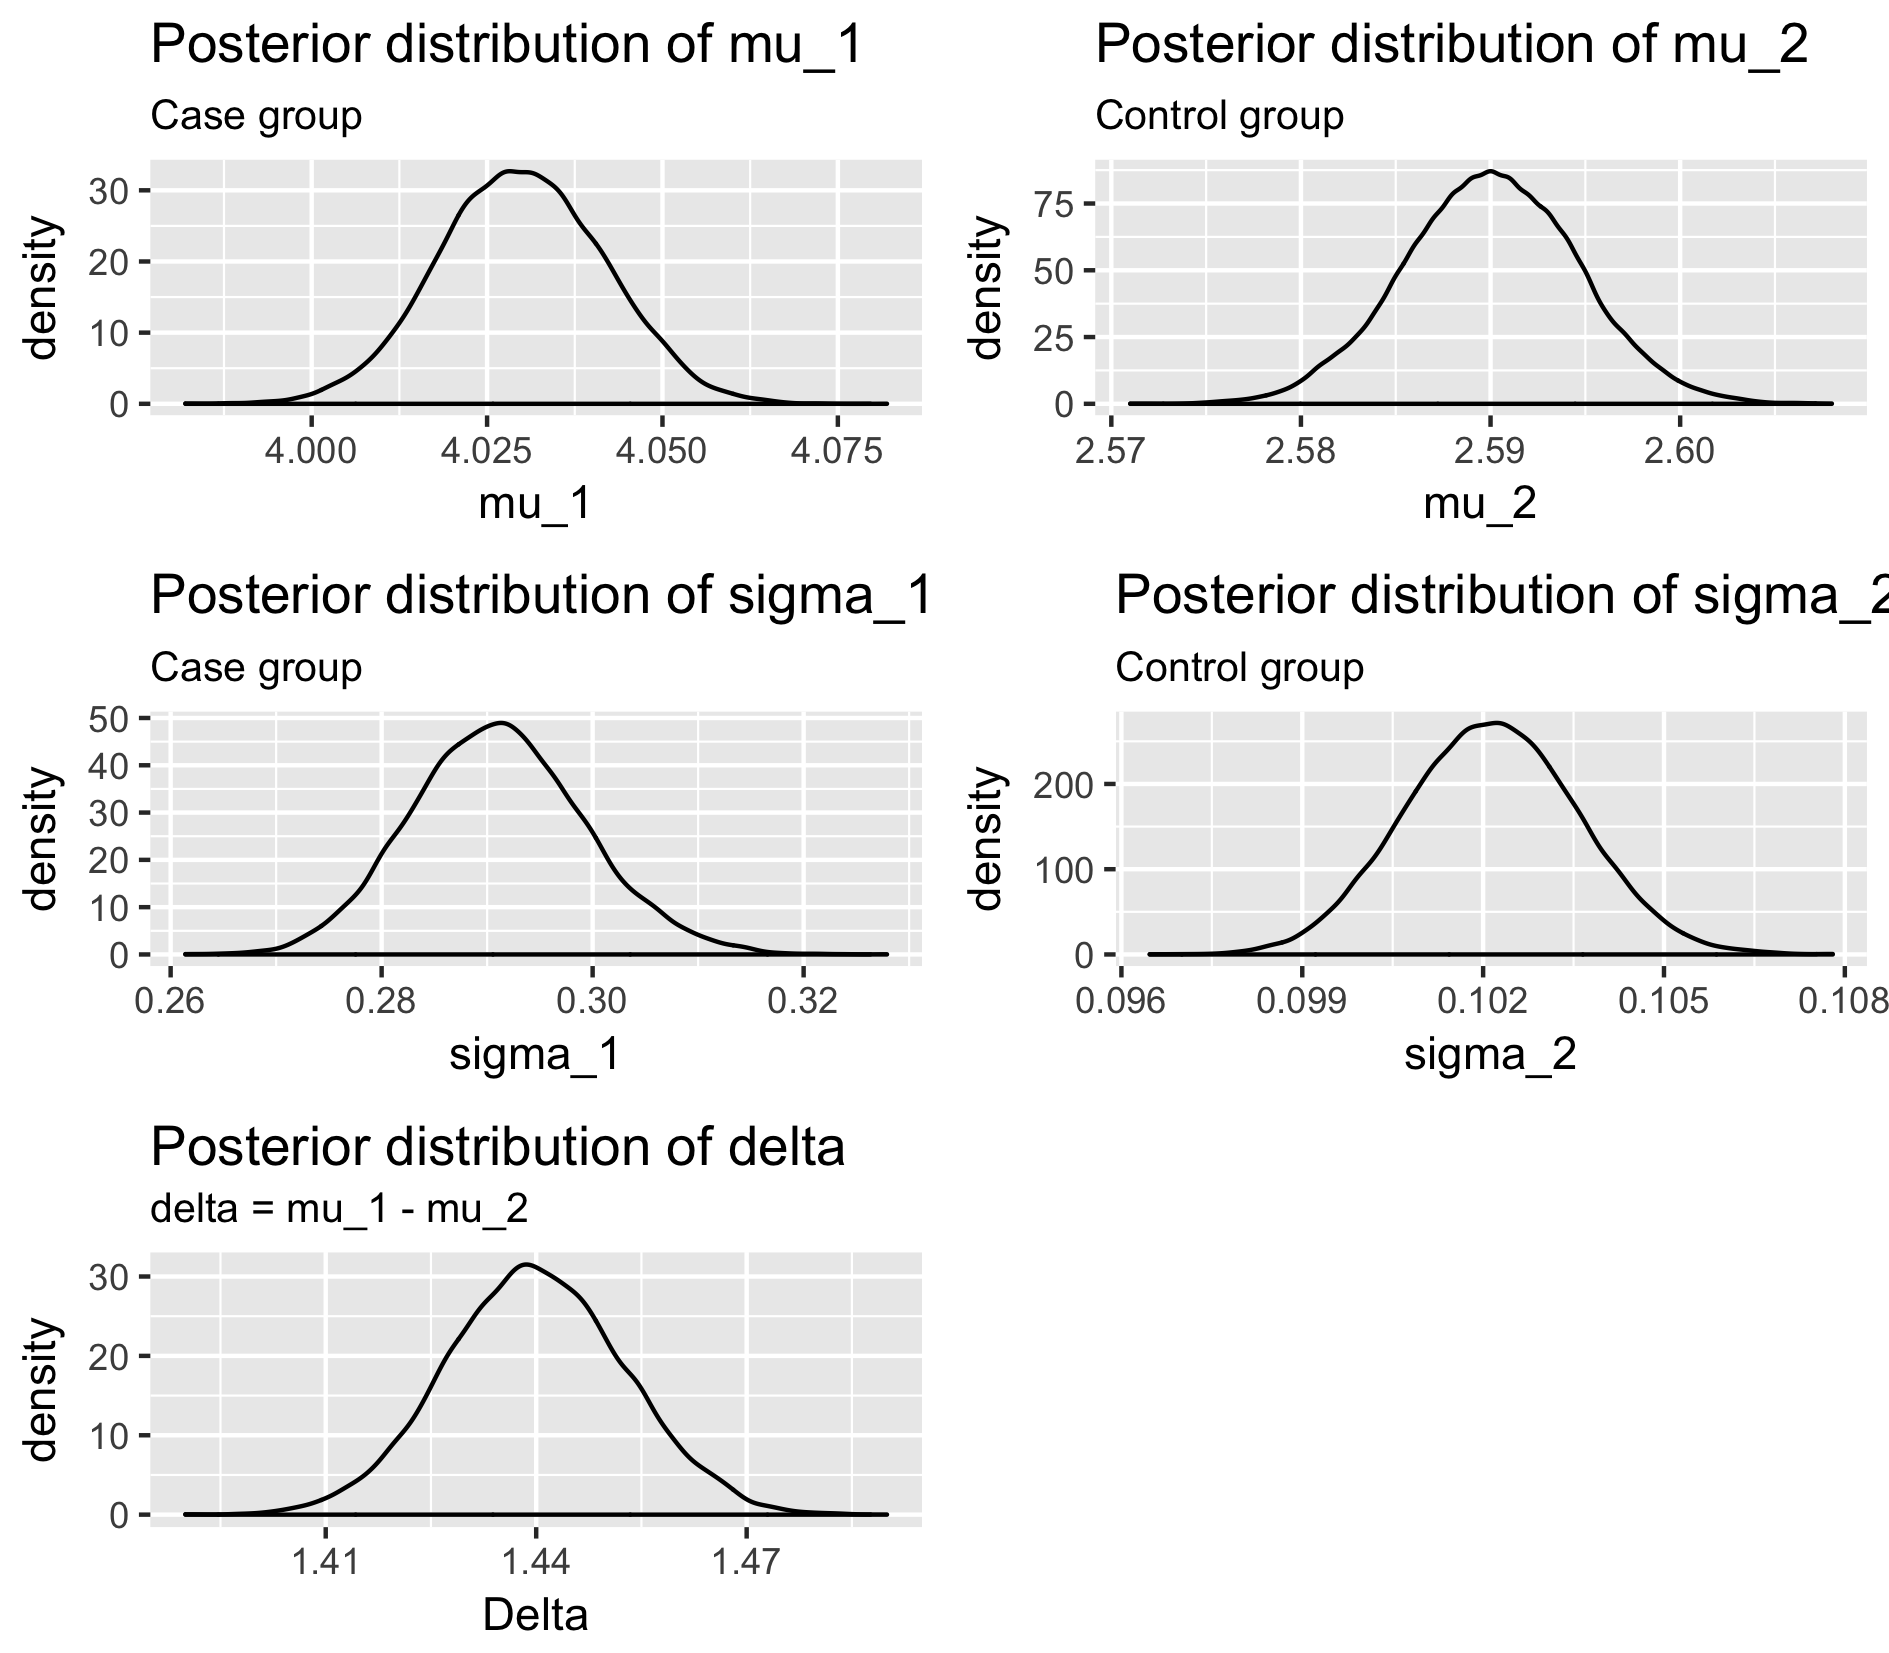
\includegraphics[width=.8\textwidth]{imgs/01_posterior_low.png}
  \caption{Posterior distributions with informative prior (low variance)}
  \label{fig:fig3}
\end{figure}

In this example, as the \cref{fig:fig3} and \cref{tbl:2} show, there is an important difference between $\mu_1$ and $\mu_2$. In fact, the credibility intervals (95\%) of each are $(4.007, 4.053)$ and $(2.581, 2.599)$ and equivalently for $\delta$: $(1.415, 1.465)$. The conclusions are the same than the previous example (with the non informative prior). But is important to distinguish that the posterior distribution of $\sigma_1$ and $\sigma_2$ are a little bit different. (0.2907 vs 0.291 and 0.1105 vs 0.1021).

\newpage
\subsubsection{Informative prior with large variance}

\begin{table}[ht!]
\centering
\caption{Summary of analysis with informative prior (large variance)}
\label{tbl:3}
\begin{tabular}{|l|lllll|}
\hline
parameters & mean   & sd     & 2.5\%  & 50\%   & 97.5\% \\ \hline
$\mu_1$    & 4.0299 & 0.0119 & 4.007  & 4.03   & 4.053  \\
$\mu_2$    & 2.59   & 0.005  & 2.58   & 2.59   & 2.6    \\
$\delta$   & 1.4399 & 0.0129 & 1.415  & 1.44   & 1.465  \\
$\sigma_1$ & 0.2907 & 0.0084 & 0.2748 & 0.2905 & 0.3081 \\
$\sigma_2$ & 0.1099 & 0.0034 & 0.1034 & 0.1099 & 0.1168 \\ \hline
\end{tabular}
\end{table}

\begin{figure}[ht!]
  \centering
  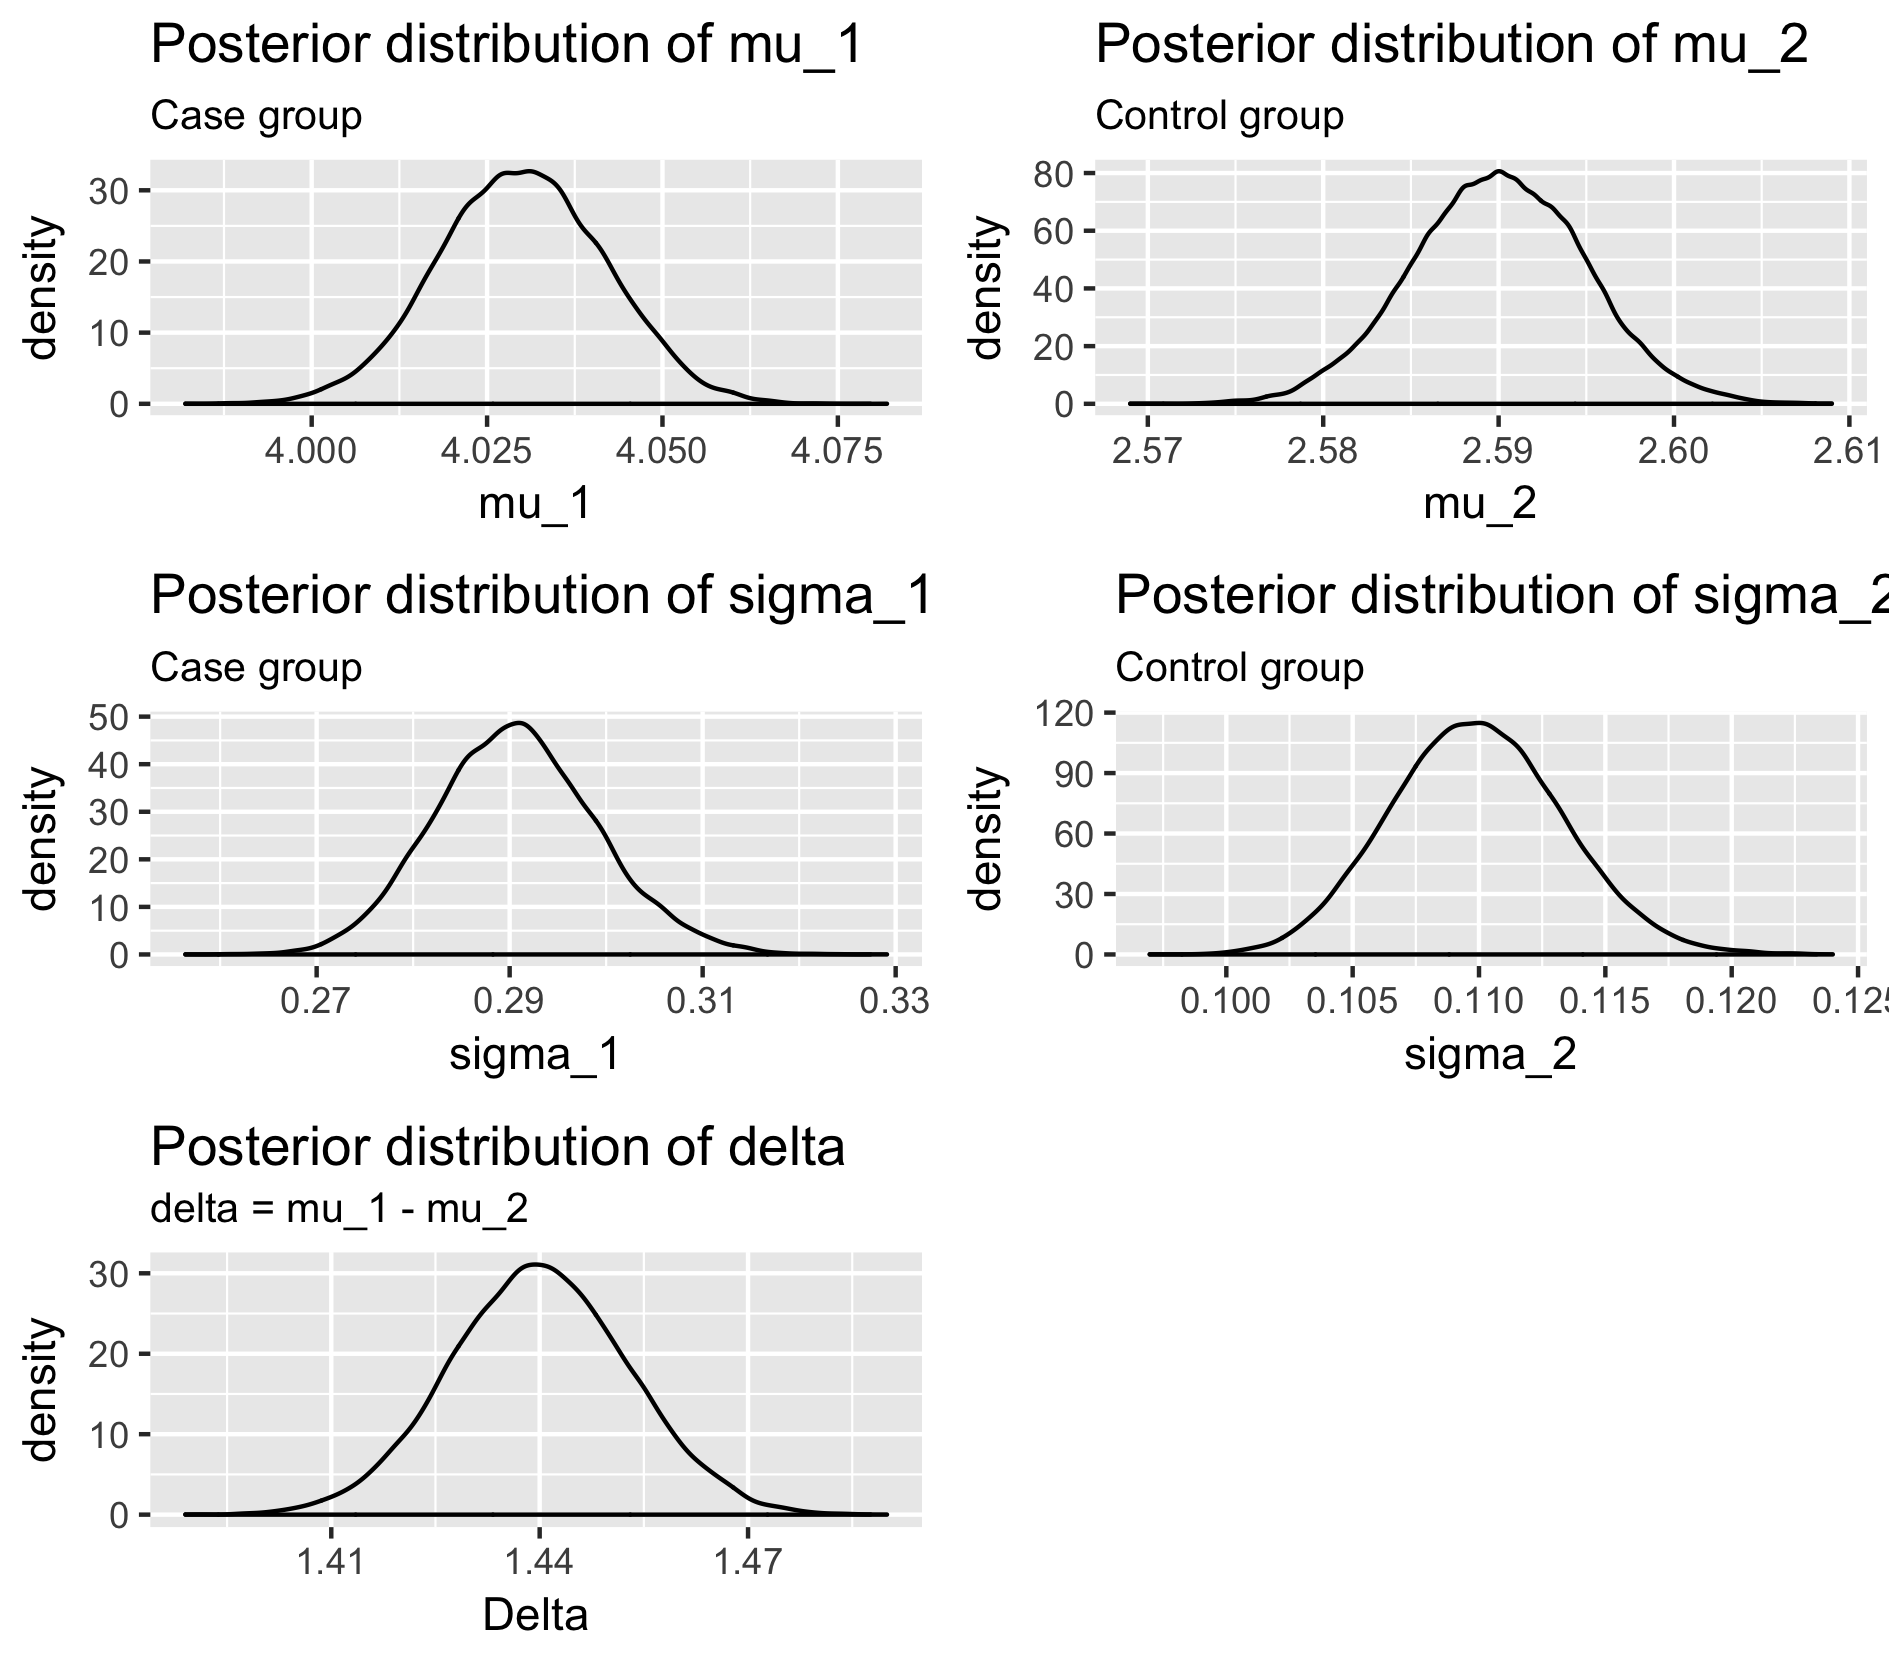
\includegraphics[width=.8\textwidth]{imgs/01_posterior_high.png}
  \caption{Posterior distributions with informative prior (large variance)}
  \label{fig:fig4}
\end{figure}

At last, the a informative a priori with large variance is used. The conclusions are the same than the previous two examples, but the estimations of the parameters and the standards deviation of them are almost the same with the first example (non informative). The differences are of the magnitude of $0.0001$.

\pagebreak
%%%%%%%%%%%%%%%%%%%%%%%%%%%%%%%%%%%%%%%%%%%%

\subsection{Posterior convergence}

For the posterior distributions showed in the last subsections, two chains were used with the initial values:
\begin{equation}
\begin{split}
\mu_1=10 \quad,\quad \mu_2 = 0 \quad,\quad \tau_1 = 0.1 \quad,\quad \tau_2 = 0.5 \\
\mu_1=-10 \quad,\quad \mu_2 = -10 \quad,\quad \tau_1 = 0.2 \quad,\quad \tau_2 = 0.2
\end{split}
\end{equation}

\subsubsection{non informative prior}

In order to determine if the chain have converged, The Gelman-Rubin statistics was tried. For the four parameters there is a good convergence, but for $\sigma_2$ maybe more iterations would be better. (There are little differences between the chains, but it is a very good convergence). Another analysis made was to check the autocorrelations coefficients. The first blue line is 1 because the lag is 0, so is the correlation between the same element. In other parts of the chain seems that there are no important correlation between the consecutive points (at least the shown).

\begin{figure}[ht!]
  \centering
  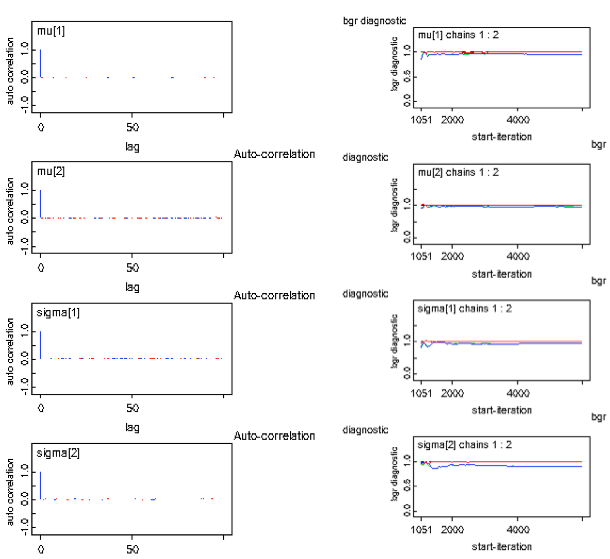
\includegraphics[width=1\textwidth]{imgs/NonInf.png}
  \caption{Autocorrelation and Gelman-Rubin statistic (non informative prior)}
  \label{fig:fig5}
\end{figure}

\pagebreak
Now, the history of the parameters is shown in \cref{fig:fig6}. Is easy to see that the chain is exploring the same area and there are almost any point outside the central area of the distributions. So, it looks very good the convergence of the chain. The burning iterations were 1500. Before that number, the chain moves trying to explore the parameters domain (different initial points should converge to the same point). This is an indication that the optimum is still not achieved, and if these iterations are considered, the analysis will be biased. The autocorrelation analysis is very important. As the MCMC name states, is a Markov Chain, so the position on the next iterations depends directly on the position in the current iteration. It is important to thin in order to de-correlate each iteration (although some authors says that most of the times it is not necessary to thinning). The MC error is good when checking the \cref{fig:fig7}. According with the BIAS project, the MC error compares with the SD of the posterior distribution in a fraction $\frac{SD}{\sqrt(iterations)}$ also that the thumb error is that should be less than $1\%$ of the posterior SD is a good value. In all the estimates this is achieved. 

\begin{figure}[ht!]
  \centering
  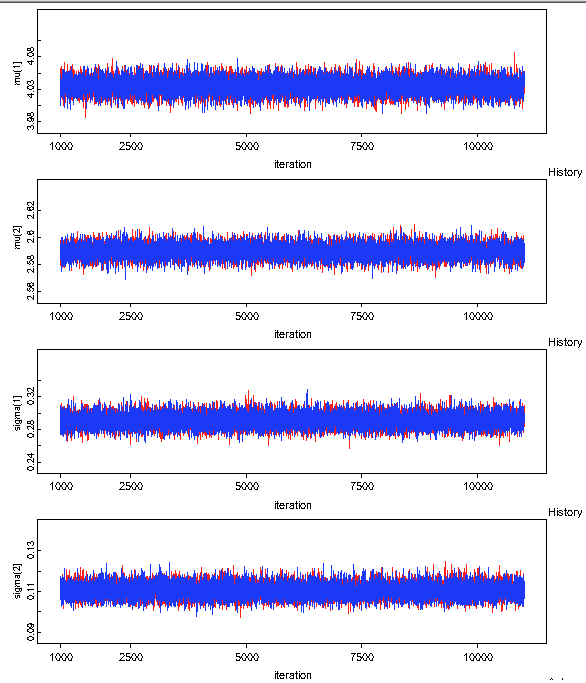
\includegraphics[width=.8\textwidth]{imgs/NonInf_hist.png}
  \caption{History of parameters (non informative)}
  \label{fig:fig6}
\end{figure}

\begin{figure}[ht!]
  \centering
  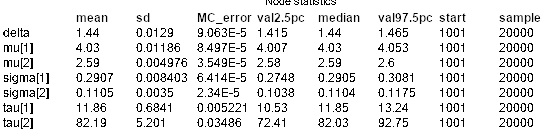
\includegraphics[width=.8\textwidth]{imgs/NonInf_table.png}
  \caption{Summary of model (non informative)}
  \label{fig:fig7}
\end{figure}

\pagebreak

%%%%%%%%%%%%%%%%%%%%%%%%%%%%%%%%%%%%%%%%%%%%
\subsection{Informative prior with low variance}
The Gelman-Rubin statistics was tried for this example too. For the four parameters there is a good convergence, but again, $\sigma_2$ could have better performance if more iterations are added. (There are little differences between the chains, but it is a very good convergence). The autocorrelation coefficients also were calculated. The conclusions are the same than the previous example.
\begin{figure}[ht!]
  \centering
  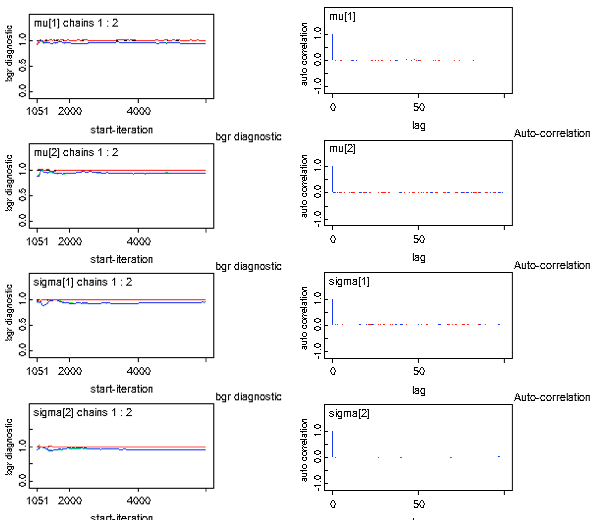
\includegraphics[width=1\textwidth]{imgs/Inf_low.png}
  \caption{Autocorrelation and Gelman-Rubin statistic (low variance prior)}
  \label{fig:fig8}
\end{figure}

\pagebreak

Again, the history of the parameters is shown in \cref{fig:fig9}. The chains seems to have converged and there is no problem associated with convergence. In this example the burning iterations were 1500 too. The values of the MC error are also below the 1\% thumb rule.

\begin{figure}[ht!]
  \centering
  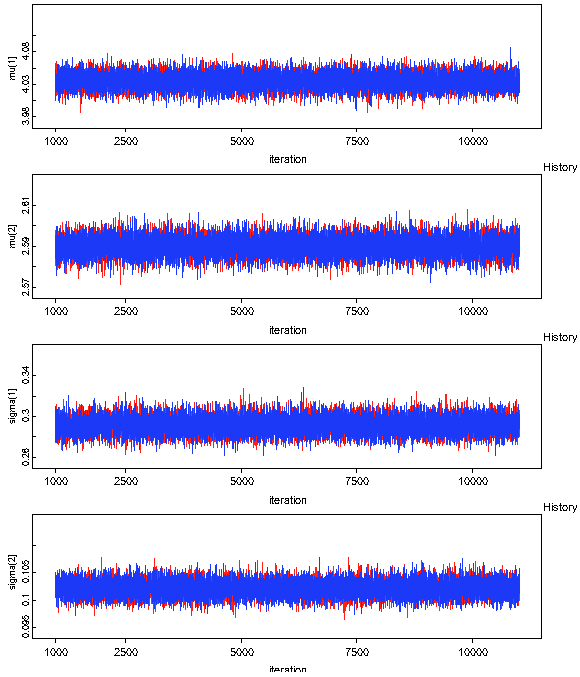
\includegraphics[width=.8\textwidth]{imgs/Inf_low_hist.png}
  \caption{History of parameters (low variance prior)}
  \label{fig:fig9}
\end{figure}

\begin{figure}[ht!]
  \centering
  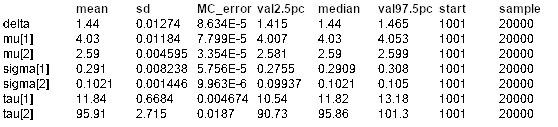
\includegraphics[width=.8\textwidth]{imgs/Inf_low_table.png}
  \caption{Summary of model (low variance prior)}
  \label{fig:fig10}
\end{figure}

\pagebreak

%%%%%%%%%%%%%%%%%%%%%%%%%%%%%%%%%%%%%%%%%%%%%%%%%%%%%%%
\subsection{Informative prior with large variance}
The Gelman-Rubin statistics was tried for this example too. For the four parameters there is a good convergence, but again, $\sigma_2$ could have better performance if more iterations are added. (There are little differences between the chains, but it is a very good convergence). The autocorrelation coefficients also were calculated. The conclusions are the same than the previous two examples.

\begin{figure}[ht!]
  \centering
  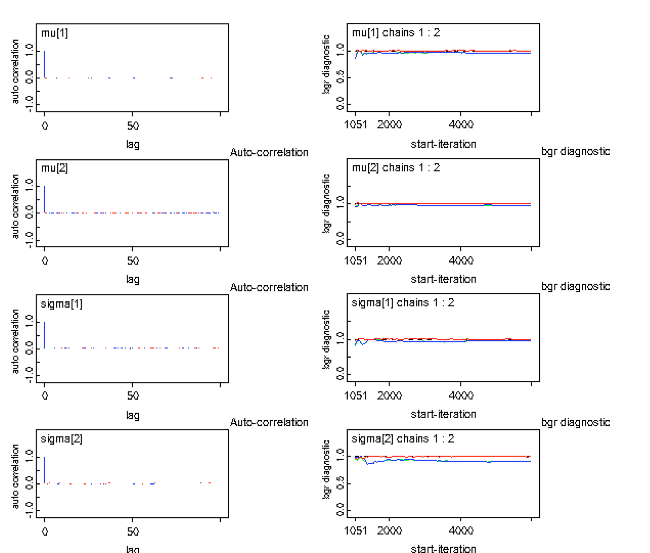
\includegraphics[width=1\textwidth]{imgs/Inf_high.png}
  \caption{Autocorrelation and Gelman-Rubin statistic (large variance prior)}
  \label{fig:fig11}
\end{figure}

\pagebreak


Again, the history of the parameters is shown in \cref{fig:fig12}. The chains seems to have converged and there is no problem associated with convergence. In this example the burning iterations were 1500 too. The values of the MC error are also below the 1\% thumb rule.

\begin{figure}[ht!]
  \centering
  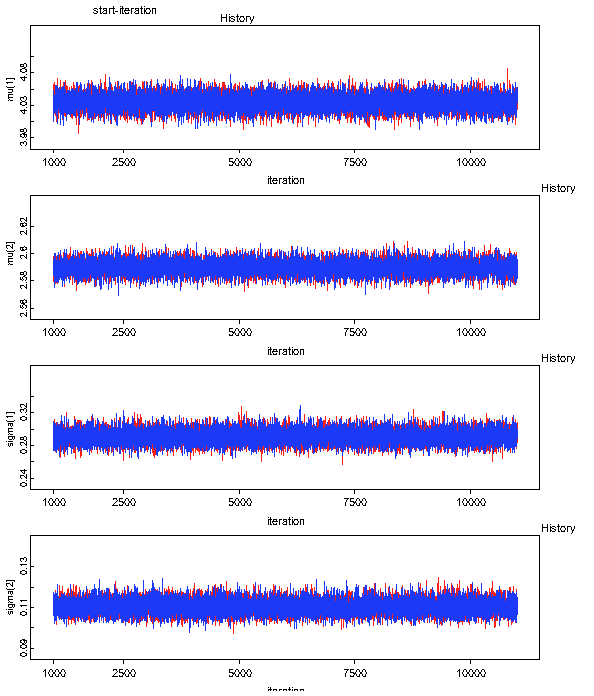
\includegraphics[width=.8\textwidth]{imgs/Inf_high_hist.png}
  \caption{History of parameters (large variance prior)}
  \label{fig:fig12}
\end{figure}

\begin{figure}[ht!]
  \centering
  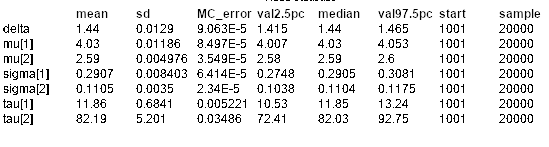
\includegraphics[width=.8\textwidth]{imgs/Inf_high_table.png}
  \caption{Summary of model (large variance prior)}
  \label{fig:fig13}
\end{figure}

\pagebreak

\section{Model comparison}
In this assignment three prior distributions were used: the first was an uninformative prior, while the second and third were informative ones. For these two, one was a distribution with low variance and the other one was a distribution with large variance. The intuition behind the apriori non informative is that this has a very large variance, so the model does not restricts the parameter into some space in the domain of the parameter. This way, a normal distribution with a very big variance can be used as a non informative prior. Now, the informative distribution with large variance is expected to behave similar than the non informative, as can be see in the \cref{fig:fig14}. Also, in this graph is easy to how is similar to the informative distribution with small variance (except in the $\sigma_2$ parameter).

\begin{figure}[ht!]
  \centering
  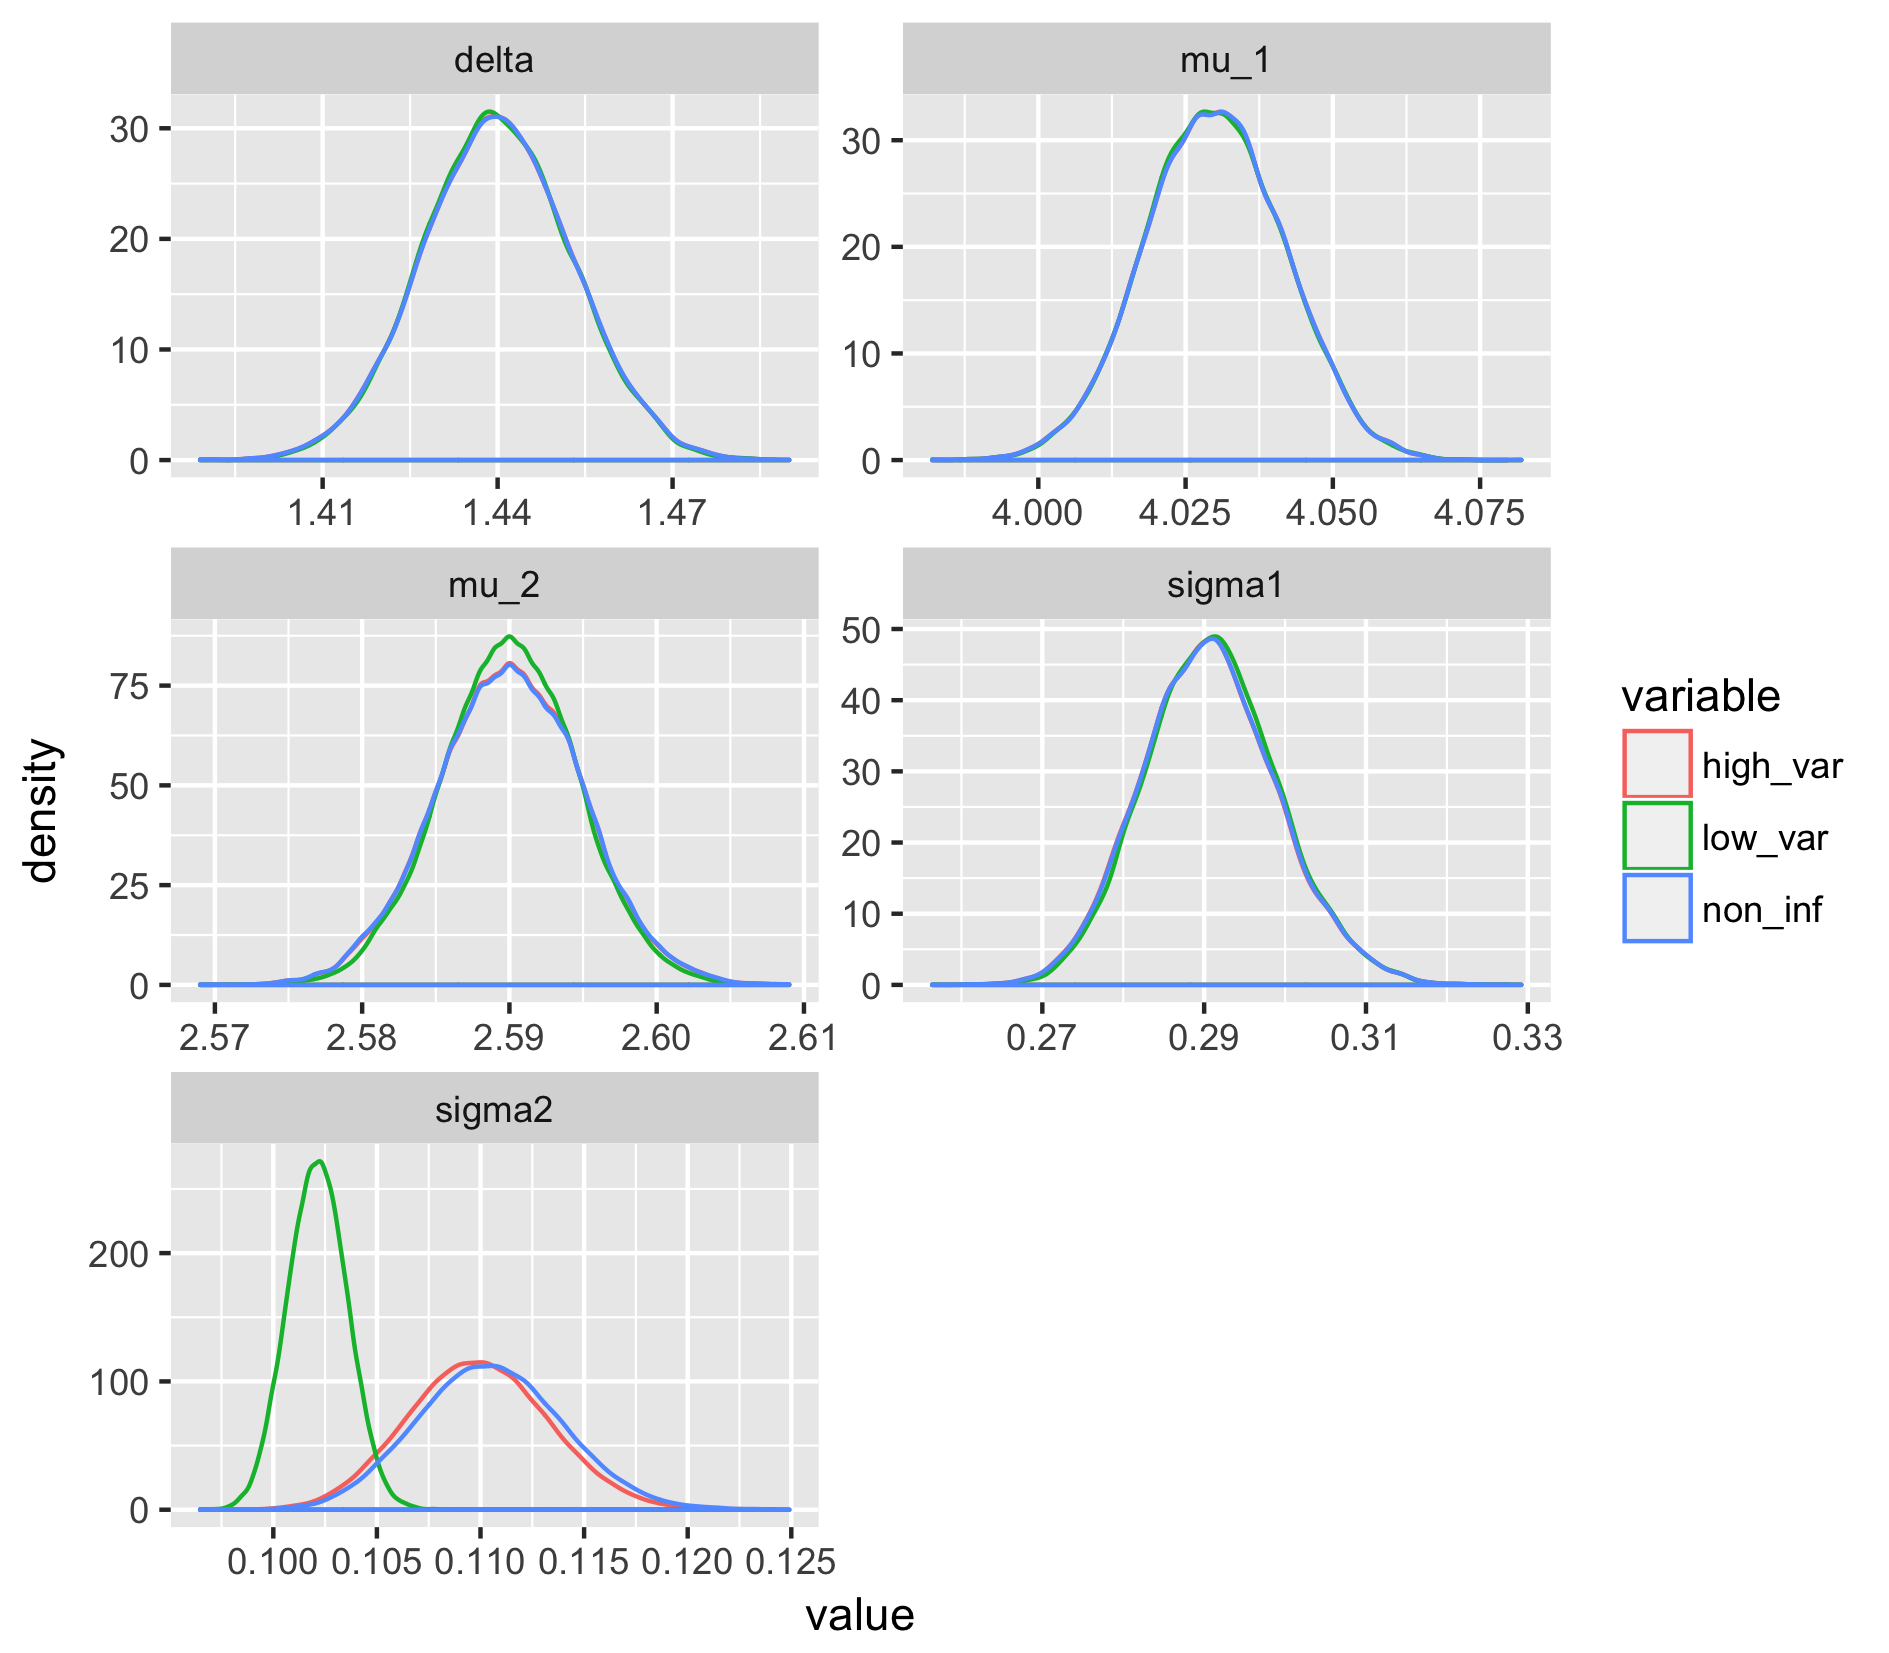
\includegraphics[width=.8\textwidth]{imgs/comparison.png}
  \caption{Comparison of posterior distributions with different apriori}
  \label{fig:fig14}
\end{figure}

Although there is a difference in $\sigma_2$, when the scale is observed, then this can be negligible (compared with the original a priori which has a mean of 100). 

In summary, the specification of a prior far from the likelihood and also with small variance, can affect the posterior distribution. But in this example it just change the mean of the distributions just by a small amount. It is important to say that the modifications of the variance can have more important changes in the posterior distribution.

\pagebreak
\appendix

\section{R graphs code}
For the plots in R, the package tidyverse and R2OpenBugs were used. Also, the package wine was used. BUGS models were sent via email

\lstinputlisting[language=R]
{/Users/salvadorgarcia/Repositories/UoE_2_BDA/12_Assignment2/01_model_noninformative.R}

Code for the comparison

\lstinputlisting[language=R]
{/Users/salvadorgarcia/Repositories/UoE_2_BDA/12_Assignment2/03_comparison.R}

\end{document}
